\documentclass{article}

\usepackage{pgf}
\usepackage{tikz}
\usetikzlibrary{arrows,automata}
\usepackage[latin1]{inputenc}
\begin{document}
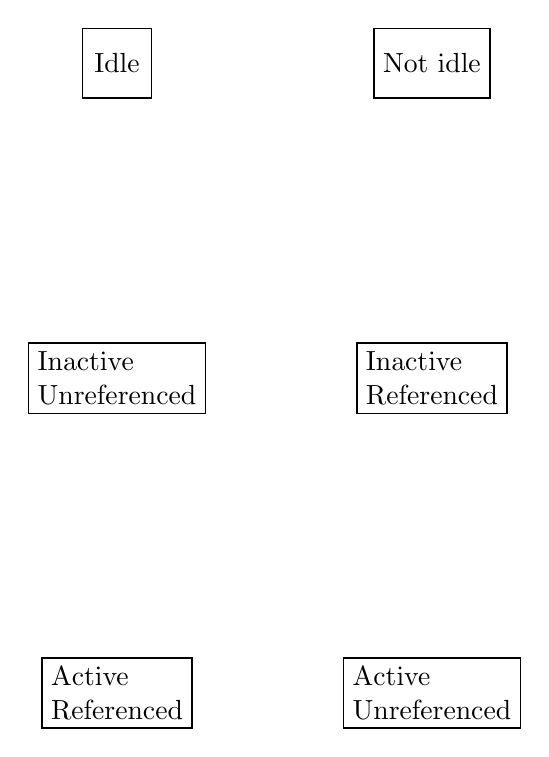
\begin{tikzpicture}[->,>=stealth',shorten >=1pt,auto,node distance=4cm,
                    semithick]
  \tikzstyle{every state}=[rectangle,draw,align=left]

  \node[state] (IU)               {Inactive \\ Unreferenced};
  \node[state] (IR) [right of=IU] {Inactive \\ Referenced};
  \node[state] (AU) [below of=IR] {Active \\ Unreferenced};
  \node[state] (AR) [below of=IU] {Active \\ Referenced};
  \node[state] (IL) [above of=IU] {Idle};
  \node[state] (NI) [right of=IL] {Not idle};

\end{tikzpicture}

\end{document}